\documentclass[10pt]{report}

\usepackage{fontspec}
\usepackage[english,frenchb]{babel}
\usepackage{titlesec}
\usepackage{titling}
\usepackage{xcolor}
\usepackage{geometry}
\usepackage{listings}
\usepackage{graphicx}
\usepackage{pgf-umlcd}
\usepackage{blindtext}

\setmainfont{Minion Pro}
\newfontfamily\headingfont{Myriad Pro}
\newfontfamily\codefont{Ubuntu Mono}

\titleformat{\chapter}[display]
{\bfseries\headingfont\filleft}
{\scalebox{0.8}[1.2] }
{0pc}
{\titlerule \vspace{0.3pc} \Huge\scalebox{0.8}[1.2]}
\titleformat{\section}[display]
{\bfseries\headingfont\filright}
{}
{0pt}
{\Large\scalebox{0.9}[1.4]}
\titlespacing{\chapter}
{0pc}{0pc}{6pc}[0pc]
\titlespacing{\section}
{0pc}{-1pc}{0pc}[0pc]


\setlength\parindent{0pt}
\setlength\parskip{6pt}

\makeatletter
\newcommand{\globalcolor}[1]{\color{#1}\global\let\default@color\current@color}
\makeatother
\definecolor{TextColor}{rgb}{0.15,0.14,0.13}
\AtBeginDocument{\globalcolor{TextColor}}

\geometry{
 a4paper, 
 voffset=0mm,
 headheight=0mm,
 headsep=0mm,
 left=17mm,
 top=26mm,
 }

\lstset{language=SQL,
		upquote=true,
        columns=flexible,
        keepspaces=true,
        breaklines,
        breakindent=0pt,
        basicstyle=\footnotesize\codefont\bfseries,
        breaklines=true,
        keywordstyle=\color{cyan},
        identifierstyle=\color{blue},
        commentstyle=\color{gray},
        stringstyle=\color{red},
        tabsize=2,
        xleftmargin=18pt,
        escapechar={¤},
        escapebegin=\color{TextColor}\normalfont\codefont,
        }

\begin{document}

\begin{titlepage}
   \vspace*{\stretch{1.0}}
   \begin{center}
   	  \Large\textbf{Projet BD avancées 2016/2017}\\
      \Large\textbf{Rapport}\\
      \large\textit{Abderrazak ZIDANE}
   \end{center}
   \vspace*{\stretch{2.0}}
\end{titlepage}

\chapter{Diagramme E/R}
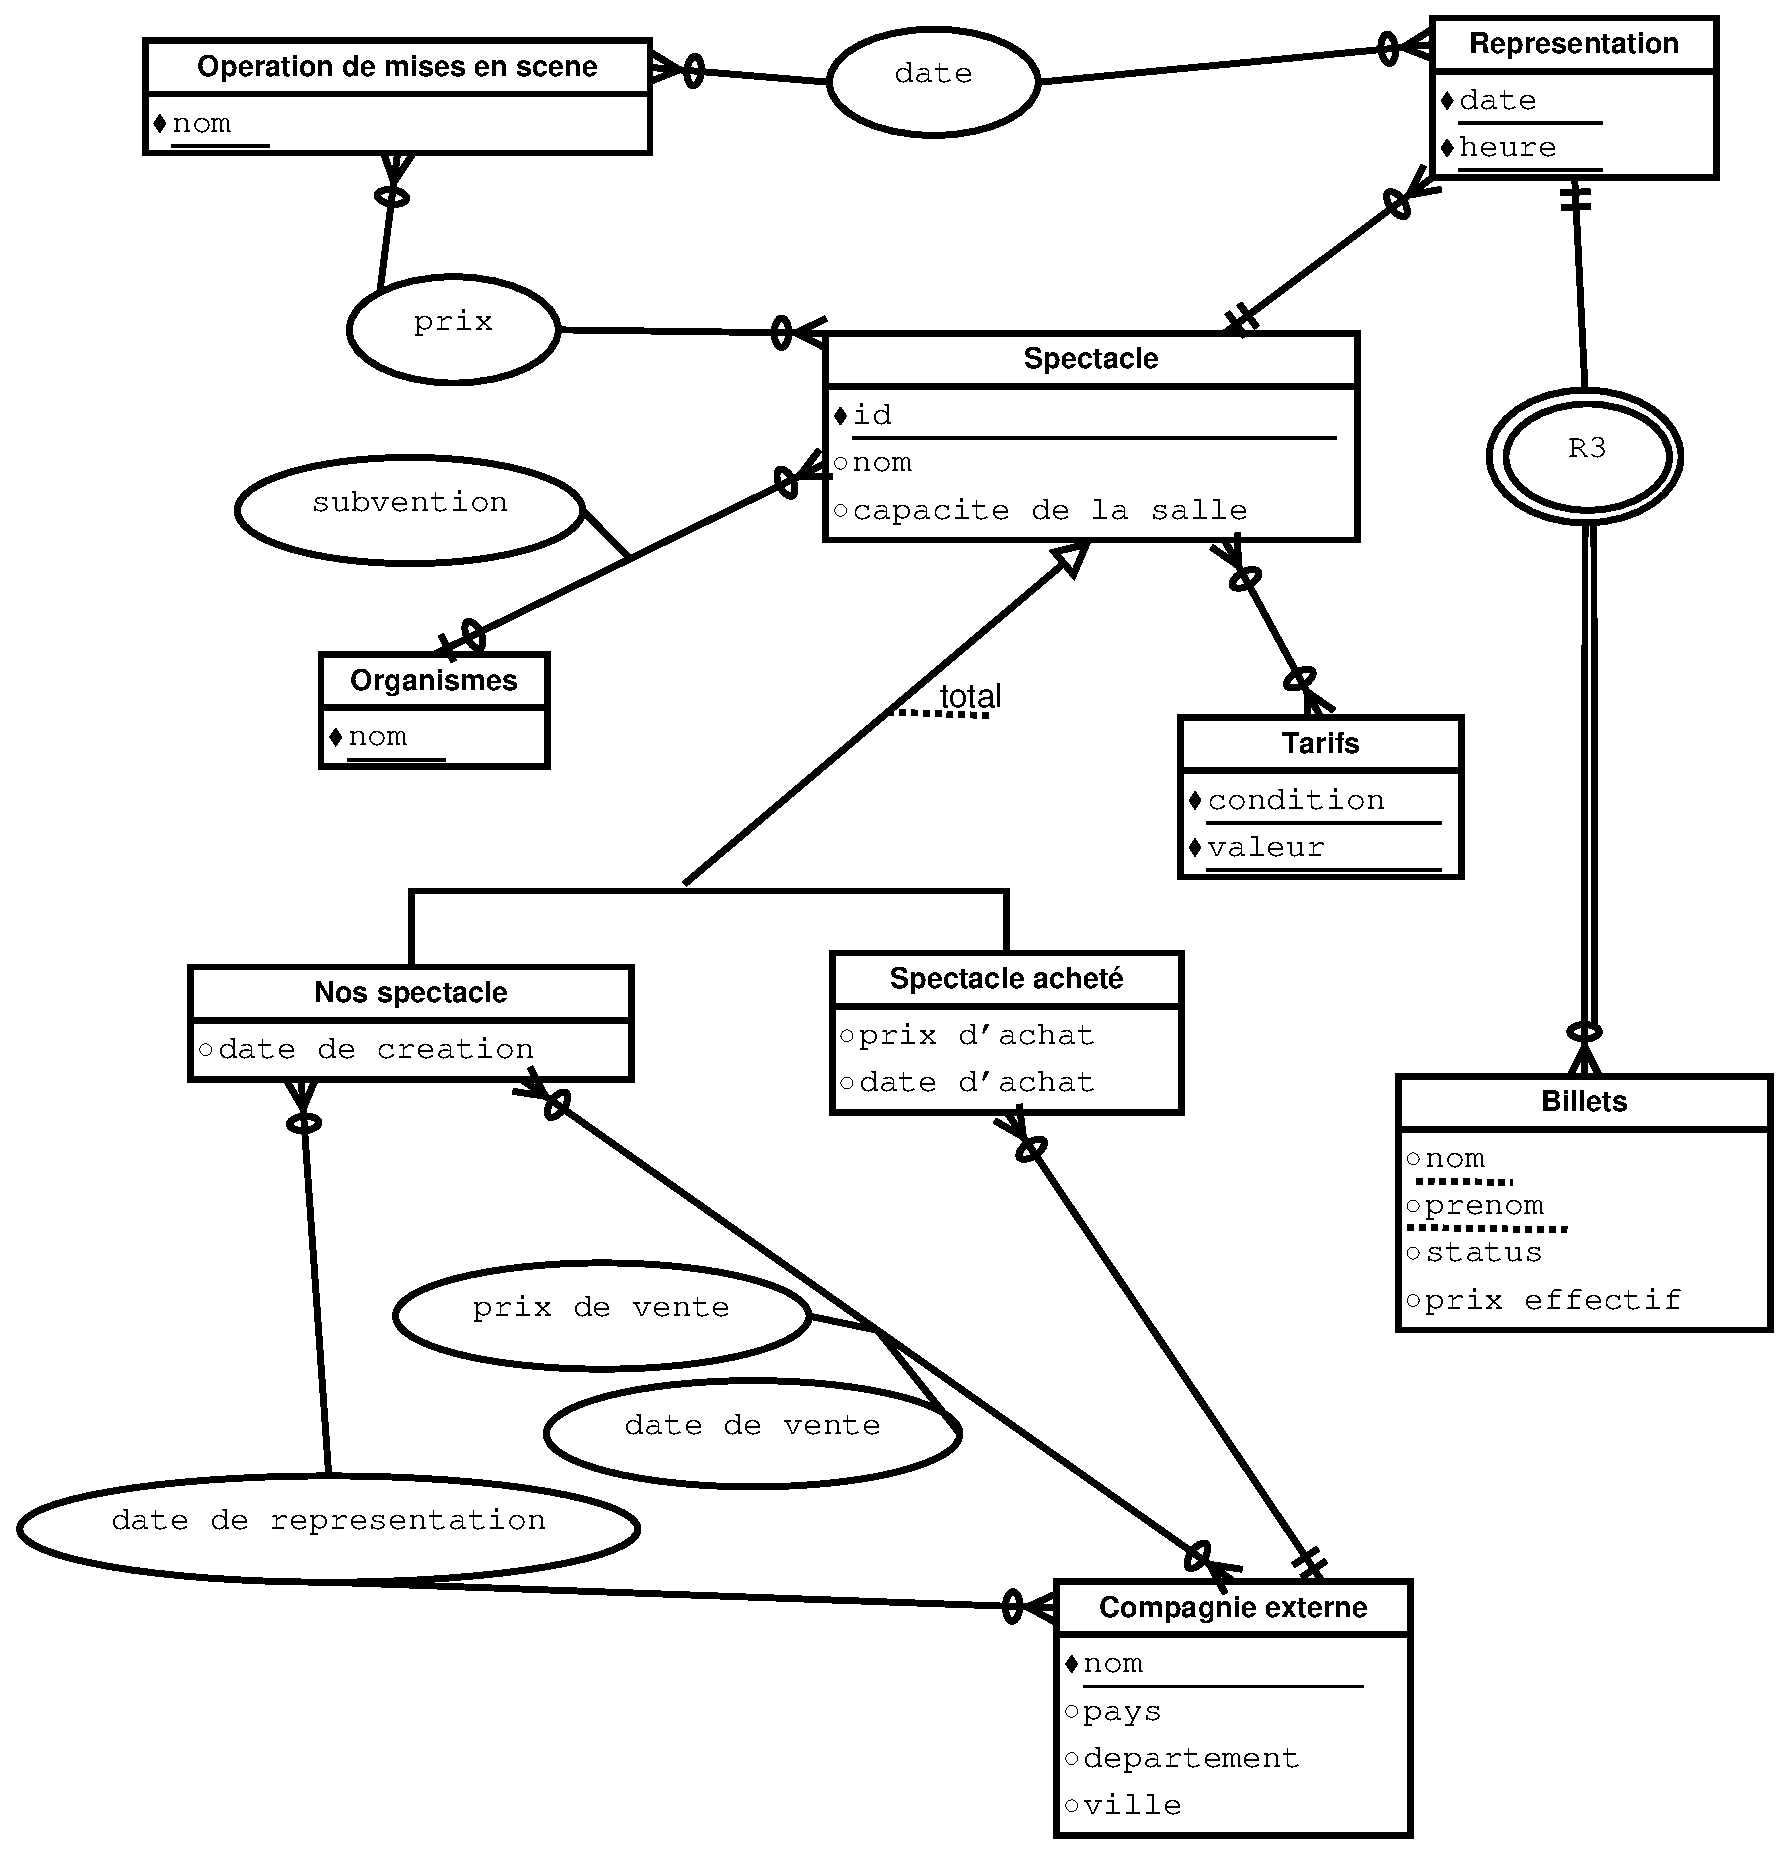
\includegraphics[width=15cm]{ER_Diagramme.eps}
\section{Contrainte externe}
\begin{itemize}
\item Le nombre de billet est la capacité de la salle
\item Une compagnie doit d,abord acheter un spectacle pour faire la représentation
\item La date d'une opération de mise en scène doit être inférieur a la date de la représentation
\end{itemize}

\chapter{Restructuration Des Spécialisation}
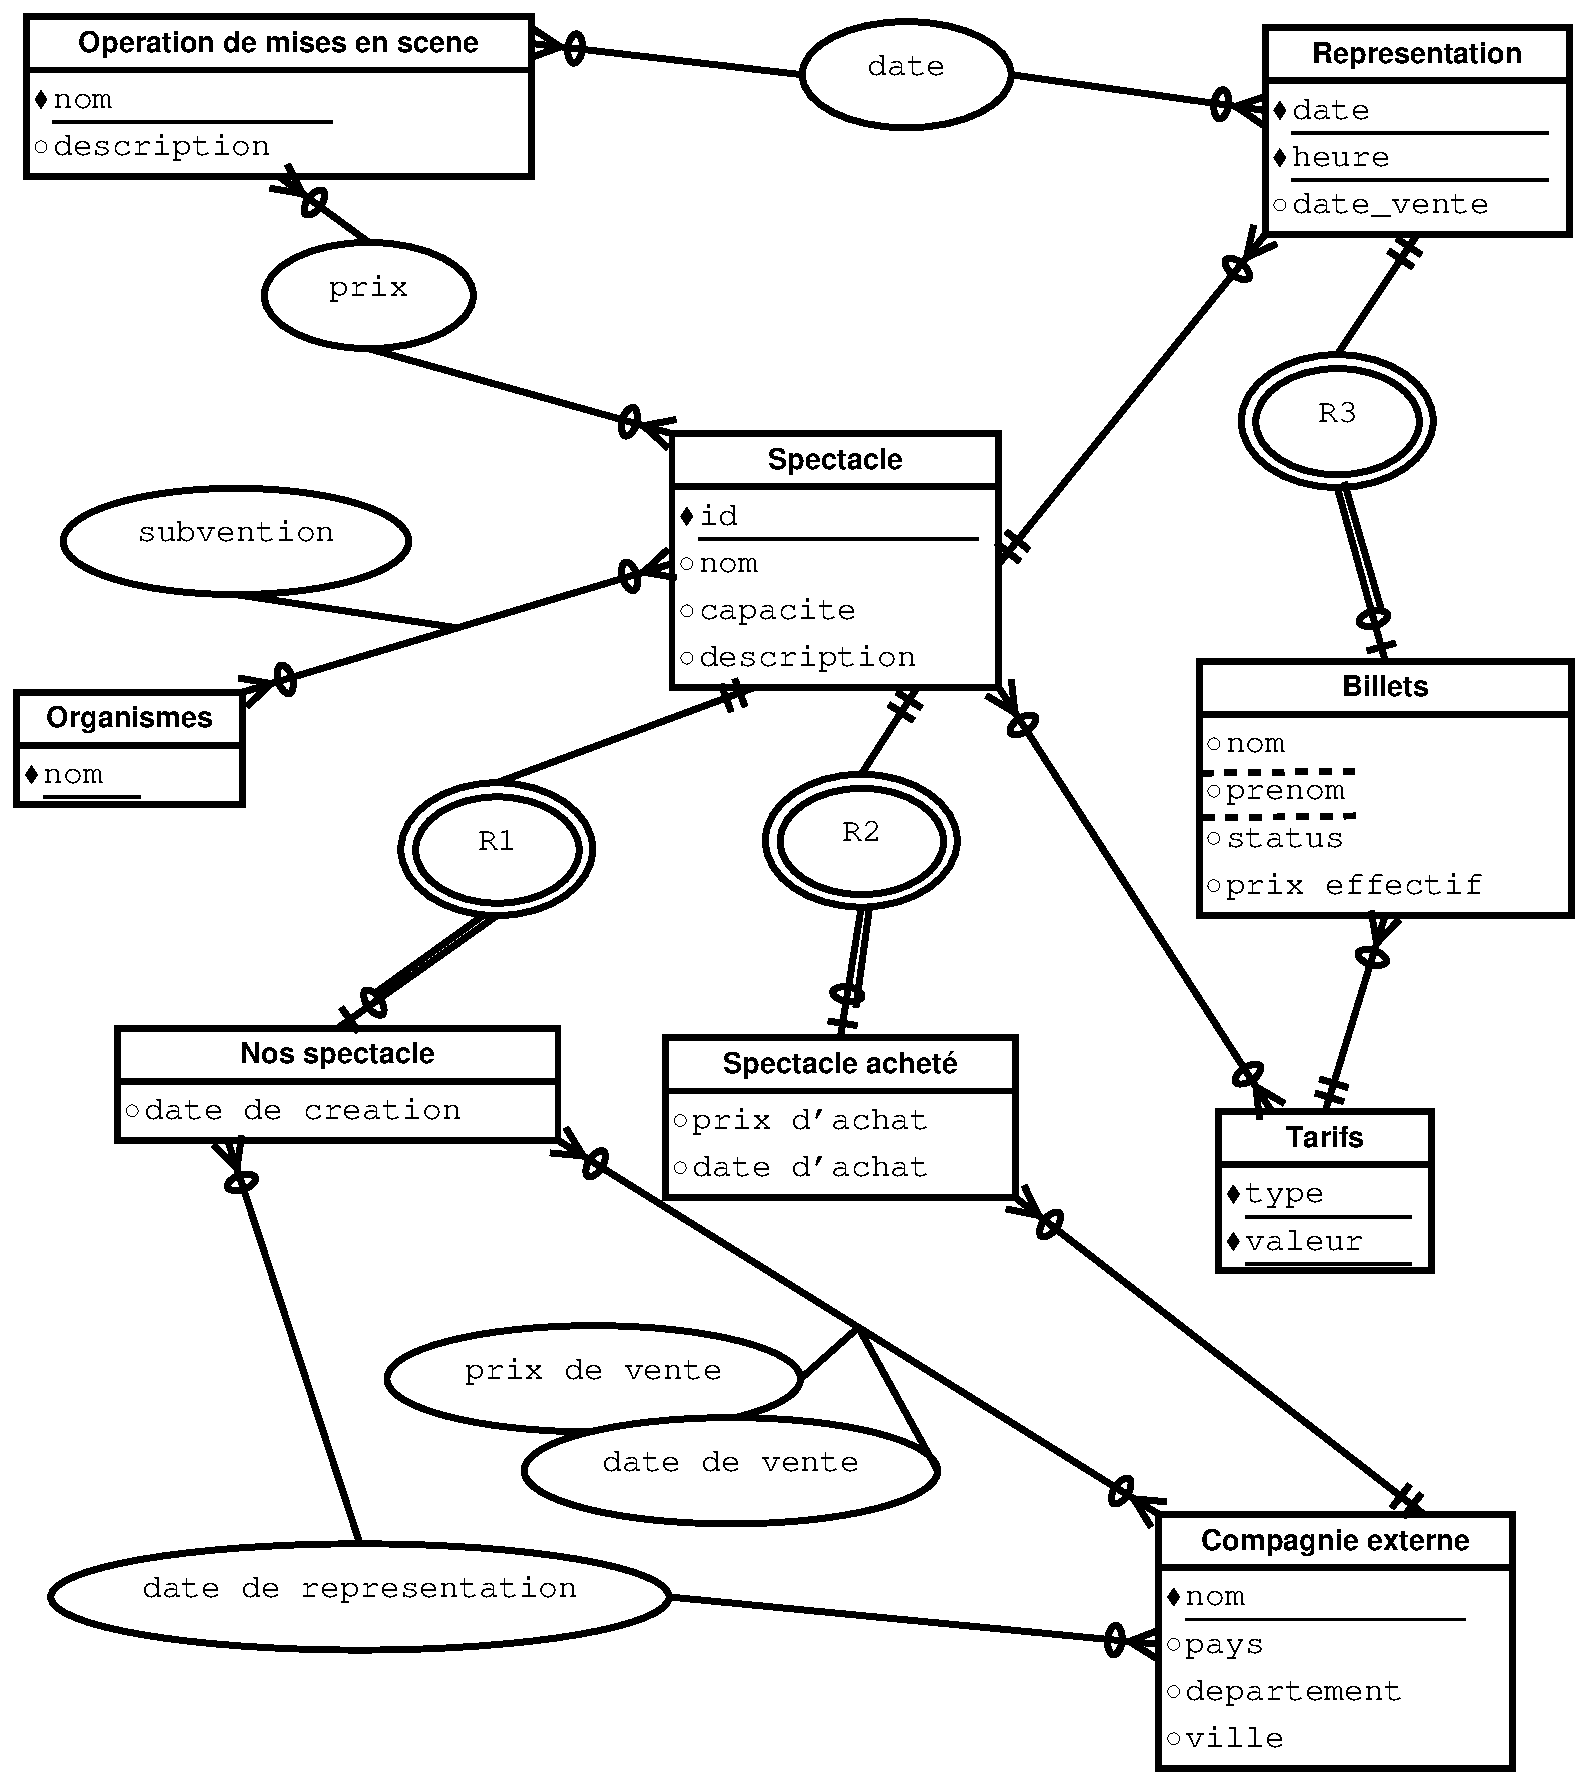
\includegraphics[width=15cm]{relationnel_diagramme.eps}
\chapter{Schéma Relationnel}
\section{Les Schéma}
\begin{itemize}
\item \textbf{spectacles}(\underline{id}, nom, capacite, description)
\item \textbf{compagnies}(\underline{nom}, pays, département, ville)
\item \textbf{spectacles\_achete}(\underline{id}, prix\_achat, date\_achat, nom\_compagnie)
\item \textbf{nos\_spectacles}(\underline{id}, date\_creation)
\item \textbf{représentations}(\underline{date\_rep, heure\_rep}, date\_vente, id\_spectacle)
\item \textbf{operations}(\underline{nom}, description)
\item \textbf{organismes}(\underline{nom})
\item \textbf{tarifs}(\underline{type\_tarif, valeur})
\item \textbf{billets}(\underline{nom, prenom, date\_rep, heure\_rep}, status, prix\_effective, type\_tarif, valeur\_tarif)

\item \textbf{op\_rep}(\underline{nom\_operation, date\_rep, heure\_rep}, date\_operation)
\item \textbf{op\_spec}(\underline{nom\_operation, id\_spectacle}, prix)
\item \textbf{opn\_com1}(\underline{id\_spectacle, nom\_compagnie}, date\_rep)
\item \textbf{opn\_com2}(\underline{id\_spectacle, nom\_compagnie}, date\_vente, prix\_vente)
\item \textbf{spec\_tar}(\underline{id\_spectacle, type\_tarif, valeur\_tarif})
\item \textbf{subventions}(\underline{id\_spectacle, nom\_organisme}, valeur)
\end{itemize}

\textbf{spectacles\_achete.id} est une clé primaire, mais aussi une clé externe vers \textbf{spectacles.id}

\textbf{nos\_spectacles.id} est une clé primaire, mais aussi une clé externe vers \textbf{spectacles.id}

2 contraintes  sur spectacle, spectacle\_acheté, nos\_spectacles

\textbf{billets.date\_rep billets.heure\_rep} est une clé externe vers \textbf{representations.date\_rep representation.heure\_rep}

\textbf{billets.type\_tarif billets.valeur\_tarifs} est une clé externe vers \textbf{tarifs.type\_tarif tarifs.valeur}

1 contraintes  sur billets, tarifs, spectacle, representation

\textbf{op\_rep.date\_rep op\_rep.heure\_rep} est une clé externe vers  \textbf{representations.date\_rep representation.heure\_rep}

\textbf{op\_rep.nom\_operation} est une clé externe vers  \textbf{operations.nom}

\textbf{op\_spec.id\_spectacle} est une clé externe vers \textbf{spectacles.id}

\textbf{op\_spec.nom\_operation} est une clé externe vers  \textbf{operations.nom}

\textbf{opn\_com1.id\_spectacle} est une clé externe vers \textbf{spectacles.id}

\textbf{opn\_com1.nom\_compagnie} est une clé externe vers \textbf{compagnies.nom}

\textbf{opn\_com2.id\_spectacle} est une clé externe vers \textbf{spectacles.id}

\textbf{opn\_com2.nom\_compagnie} est une clé externe vers \textbf{compagnies.nom}

\textbf{spec\_tar.id\_spectacle} est une clé externe vers \textbf{spectacles.id}

\textbf{spec\_tar.type\_tarif spec\_tar.valeur\_tarifs} est une clé externe vers \textbf{tarifs.type\_tarif tarifs.valeur}

\textbf{subventions.id\_spectacle} est une clé externe vers \textbf{spectacles.id}

\textbf{subventions.nom\_organisme} est une clé externe vers \textbf{organismes.nom}

\chapter{PostgreSQL programme}
\section{Créé la base de donnée}
\begin{lstlisting}
CREATE DATABASE "THEATRE"
WITH 
OWNER = postgres
ENCODING = 'UTF8'
CONNECTION LIMIT = -1;
\end{lstlisting}

\section{Créé les tables}
\begin{lstlisting}
DROP TABLE IF EXISTS spectacles_achete;
DROP TABLE IF EXISTS nos_spectacles;
DROP TABLE IF EXISTS billets;
DROP TABLE IF EXISTS op_rep;
DROP TABLE IF EXISTS representations;
DROP TABLE IF EXISTS op_spec;
DROP TABLE IF EXISTS opn_com1;
DROP TABLE IF EXISTS opn_com2;
DROP TABLE IF EXISTS spec_tar;
DROP TABLE IF EXISTS subventions;
DROP TABLE IF EXISTS spectacles;
DROP TABLE IF EXISTS compagnies;
DROP TABLE IF EXISTS operations;
DROP TABLE IF EXISTS organismes;
DROP TABLE IF EXISTS tarifs;

CREATE TABLE spectacles (
id              int	primary key not null,
nom         	text not null,           
capacite        real not null,          
description     text
);

CREATE TABLE compagnies (
nom             text primary key not null,
pays      		text not null,           
departement     text not null,          
ville  			text not null
);

CREATE TABLE spectacles_achete (
id              int	primary key not null REFERENCES spectacles,
prix_achat      real not null,           
date_achat      date not null,          
nom_compagnie   text not null REFERENCES compagnies
);

CREATE TABLE nos_spectacles (
id              int	primary key not null REFERENCES spectacles,
date_creation   date not null
);

CREATE TABLE representations (
date_rep    date not null,
heure_rep   time not null,
date_vente  date not null,
id_spectacle int not null REFERENCES spectacles, 
PRIMARY KEY (date_rep, heure_rep)
);


CREATE TABLE operations (
nom             text primary key not null,
description		text
);

CREATE TABLE organismes (
nom             text primary key not null
);

CREATE TABLE tarifs (
type_tarif        text not null,
valeur             real not null,
PRIMARY KEY (type_tarif, valeur)
);

CREATE TABLE billets (
nom        				text not null,
premon     				text not null,
date_rep      			date not null,
heure_rep      			time not null,
status     				text not null,
prix_effective     		text not null,
type_tarif	     		text not null,
valeur_tarif    		real not null,
PRIMARY KEY (nom, premon, date_rep, heure_rep),
FOREIGN KEY (date_rep, heure_rep) REFERENCES representations(date_rep, heure_rep),
FOREIGN KEY (type_tarif, valeur_tarif) REFERENCES tarifs(type_tarif, valeur)
);

CREATE TABLE op_rep (
nom_operation   text not null REFERENCES operations,
date_rep    	date not null,
heure_rep   	time not null,
date_operation        date not null,
PRIMARY KEY (nom_operation, date_rep, heure_rep),
FOREIGN KEY (date_rep, heure_rep) REFERENCES representations(date_rep, heure_rep)
);

CREATE TABLE op_spec (
nom_operation   text not null REFERENCES operations,
id_spectacle int not null REFERENCES spectacles,
prix real not null
);


CREATE TABLE opn_com1 (
id_spectacle int not null REFERENCES spectacles,
nom_compagine   text not null REFERENCES compagnies,
date_rep date not null
);

CREATE TABLE opn_com2 (
id_spectacle int not null REFERENCES spectacles,
nom_compagine   text not null REFERENCES compagnies,
date_vente date not null,
prix_vente real not null
);

CREATE TABLE spec_tar (
id_spectacle int not null REFERENCES spectacles,
type_tarif	     		text not null,
valeur_tarif    		real not null,
FOREIGN KEY (type_tarif, valeur_tarif) REFERENCES tarifs(type_tarif, valeur)
);

CREATE TABLE subventions (
id_spectacle int not null REFERENCES spectacles,
nom_organisme   text not null REFERENCES organismes,
valeur real not null
);
\end{lstlisting}
\chapter{Triggers}
\section{Contrainte externe sur billet}
les champs type\_tarifs  et valeur\_tarifs présent dans la table billets, doivent être lié a la table spectacle
\begin{lstlisting}
CREATE FUNCTION verifie_tarif_du_spectacle() RETURNS trigger AS $$ 
DECLARE id_s int;
BEGIN
SELECT id_spectacle INTO id_s FROM representations WHERE date_rep = NEW.date_rep AND heure_rep = NEW.heure_rep;
SELECT * FROM spec_tar WHERE id_spectacle = id_s AND type_tarif = NEW.type_tarif AND valeur_tarif = NEW.valeur_tarif;
IF NOT FOUND THEN RETURN NULL;
END IF;
RETURN NEW;
END; 
$$ LANGUAGE plpgsql;


CREATE TRIGGER tarifs_billets
BEFORE INSERT OR UPDATE ON billets
FOR EACH ROW
EXECUTE PROCEDURE verifie_tarif_du_spectacle();
\end{lstlisting}

\section{Contrainte externe sur nos\_specacles}
si un spectacle est présent dans nos\_spectacle, il doit pas être présent dans spectacles\_achete
\begin{lstlisting}
CREATE FUNCTION verifie_spectacle_is_not_achete() RETURNS trigger AS $$ 
DECLARE id_s int;
BEGIN
SELECT id INTO id_s FROM spectacles_achete WHERE id = NEW.id;
IF NOT FOUND THEN RETURN NEW;
END IF;
RETURN NULL;
END; 
$$ LANGUAGE plpgsql;


CREATE TRIGGER spectacle
BEFORE INSERT OR UPDATE ON nos_spectacles
FOR EACH ROW
EXECUTE PROCEDURE verifie_spectacle_is_not_achete();
\end{lstlisting}

\section{Contrainte externe sur spectacles\_achete}
si un spectacle est présent dans spectacles\_achete, il doit pas être présent dans nos\_spectacle
\begin{lstlisting}
CREATE FUNCTION verifie_spectacle_is_nos() RETURNS trigger AS $$ 
DECLARE id_s int;
BEGIN
SELECT id INTO id_s FROM nos_spectacles WHERE id = NEW.id;
IF NOT FOUND THEN RETURN NEW;
END IF;
RETURN NULL;
END; 
$$ LANGUAGE plpgsql;

CREATE TRIGGER spectacle
BEFORE INSERT OR UPDATE ON spectacles_achete
FOR EACH ROW
EXECUTE PROCEDURE verifie_spectacle_is_nos();
\end{lstlisting}

\section{Politiques tarifaires}
si un spectacle est présent dans spectacles\_achete, il doit pas être présent dans nos\_spectacle
\begin{lstlisting}

\end{lstlisting}

\end{document}